\documentclass[
  final,
  babelLanguage=british,
  desktopVersion,
  %showtrims,
  %overleaf,
]{anecdote}

%\graphicspath{{./assets/photos/300dpi/}}
\graphicspath{{./assets/photos/92dpi/}}

% Page size: 135 x 120 mm
% Body text: 11 / 14 pt

\usepackage{local}

%% Details of the book
%% ===================

\title{Meditation Without the Hurry}
\subtitle{-- but with the grit.}
\author{Gambhīro Bhikkhu}
\publisher{The Publisher}% TODO
\date{2019-10-04}
\editionInfo{\textit{First edition}, 2019}% TODO update edition info
\ISBN{000-000-0000-00-0}% TODO update ISBN

% === Metadata ===

\hypersetup{
  pdftitle={\thetitle},
  pdfauthor={\theauthor},
  pdfcopyright={Copyright (C) 2019, \thePublisher},
  pdfsubject={},% TODO subject
  pdfkeywords={},% TODO keywords
  pdflicenseurl={https://creativecommons.org/licenses/by-nc-nd/4.0/},
  pdfcontacturl={},
  pdflang={en},
}

%% === Load further packages ===

%% === Hyphenation exceptions and corrections ===

\hyphenation{London}

\begin{document}

\frontmatter

\ifdesktopversion
\desktopCover{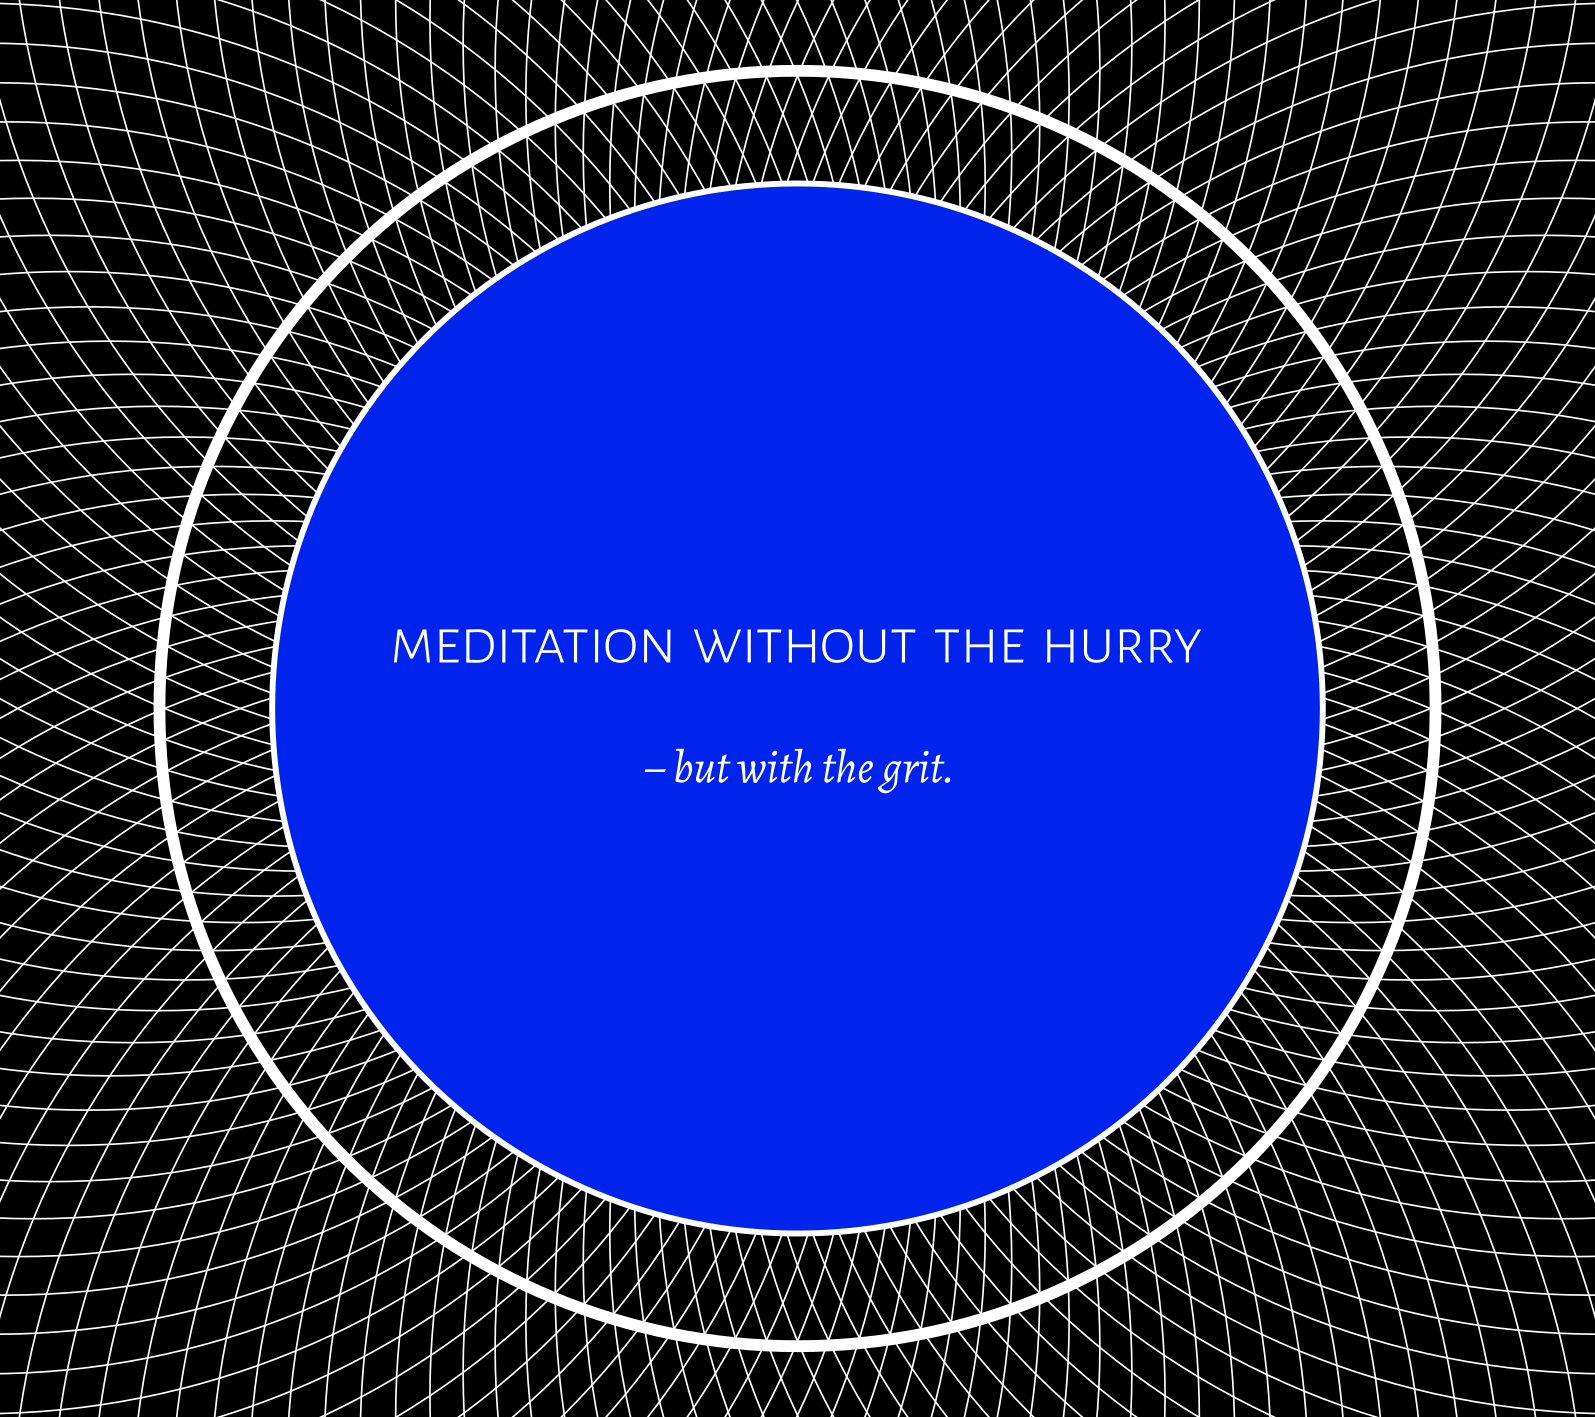
\includegraphics[height=\paperheight]{./desktop-cover-en.png}}
\fi

\cleartorecto
\thispagestyle{empty}
\vspace*{5em}

{\centering

{\Large\alegreyaSansScLightFont\selectfont\MakeLowercase{\textls*{\thetitle}}}\\[5pt]
{\chapterTitleFont\selectfont\itshape \thesubtitle}

\vfill

{\chapterTitleFont \theauthor}

\vspace*{2em}

}



\cleartoverso
\thispagestyle{empty}

{\copyrightsize
\centering
\setlength{\parindent}{0pt}%
\setlength{\parskip}{0.8\baselineskip}%

\thetitle\\
by \theauthor

% Published by \thePublisher
% 
% ISBN \theISBN
% 
% Copyright \copyright\ \thePublisher\ 2019
% 
% Cover Photograph: The Person

\vfill

This work is licensed under a Creative Commons\\
Attribution-NonCommercial-NoDerivatives 4.0 International~License.

Produced with the \LaTeX\ typesetting system, set in Crimson Roman and Alegreya Sans.

% \theEditionInfo

}


\cleartorecto
\thispagestyle{empty}

\mbox{}\vfill

\noindent
{\itshape
  \ldots\ The wise acts without haste,\\
  teaches without words,\\
  lets the waters flow, doesn't struggle\ldots
}

\bigskip

\noindent
{\smaller Tao Te Ching}

\vfill\mbox{}


\cleartorecto
\tableofcontents*

%\input{./manuscript/tex/foreword.tex}

%\input{./manuscript/tex/preface.tex}

% Page 1 is the first page of the first chapter.
\mainmatter

\hypertarget{breathing-1}{%
\chapter{Breathing}\label{breathing-1}}

We watch the sensations of the breathing in the body, this alert
attention collects and calms the mind. We watch, what do we feel in the
body when we breathe in, what do we feel when we breathe out.

Breathing in, we feel the cold air first at the tip of the nose, it
fills the lungs while the chest expands and the abdomen draws in
slightly. There is no need to control this. The body knows how to
breathe, for us it is enough to observe, like watchings waves wash in
onto the shore, and then recede.

We don't have to tell ourselves what to think and how to feel. If we
want clear thoughts, it is best to first be silent and listen. We sit
quietly for a little while, and when we are silent, the clear thoughts
will come their own, or the mind will be satisfied with the silence.

A clear, conscios thought is followed by peaceful gladness, the mind is
content and happy, doesn't feel the need for a lot of internal
discussion, it is satisfied to listen to the silence.

The right attitude is a careful balance. We establish a clear intention
to stay with the meditation and leave other matters until a later time,
but too much force becomes rigid and obstructive.

A clear mind and good aspiration feels settled and cool, open for
changes. A struggle of will-power feels busy and hot, narrow in scope.

I remember, I used to think that during meditation we are observing the
breathing because we are supposed to learn new things from it. I sat
down and struggled to understand how to do it, and kept thinking and
changing how to breathe, expecting that eventually it will somehow work,
and some day, doing it in the right way I will start learning new facts
about the mind. It was rather painful and mostly fruitless.

The best is when we have to learn something we didn't volunteer to
learn. We don't learn new facts from meditation, because there are so
few that we need, that we probably already know them.

But we don't stop to stay with them, and unpack their significance for
\emph{what to do}, \emph{in what manner to do it}, or in other words
\emph{how to be}. A list of facts, if not integrated, doesn't reach deep
enough to deal with root causes in the heart and mind, and have no
effect on us. Watching the breath stops us and opens the attention which
can do that.

The Buddha only has a simple message for us: wake up, stop holding on,
you don't have to suffer. We keep unpacking this, opening it wider and
wider.

Take a few minutes to adjust how you sit and find a balanced posture.
The important point is to be upright, in a stable but not tense posture,
with the head balanced and not lulling forward, and that your posture
should allow open, easy breathing.

Determine that you are putting down everyday activities for this period.
If such a thought interrupts you, respond, 'This is not the right time,
I will come back to that when the time is appropriate. At this time, I
am watching the body the breathing.' It's a bit longer than 'Go away!',
but more friendly to ourselves. It helps to think the thought
deliberately. This establishes a clear intention in the mind, like
clearing a desk before starting work. We are putting them down not
because they are not important, but because we care about doing our
tasks well. If we don't rest, we can't do our work well.

Take a deep breath and watch if you feel tension, something obstructing
or limiting the breath. If it moves easy and open, then your posture is
suitable. You don't have to sit in a special way.

Pay attention to the physical sensation of breathing. Let the body
regulate the breath, we only watch and let it relax, giving attention to
what is happening now.

Good posture and the calm, easy breathing is a quiet and pleasant
feeling, like sitting down on a park bench after a walk. There nothing
special to do, and this simple, quiet sitting is a joy in itself.

Breathing in, we first feel the air at the nostril. The cold air moves
down in the windpipe, fill the lungs, and the chest expands. The abdomen
muscles and diaphragm move inward and outward, controlling the movement
of the air. The quiet rhythm of heartbeats can be felt. Breathing out,
the muscles relax, the chest contracts and the rib bones move closer.
The warm air rises through the wind pipe, and exits the body through the
nose.

It is not necessary to express this in thought, relax and watch as the
feelings appear in the body. It takes a few minutes for the body to
settle. The beating of the heart will calm down, and the breathing will
become regular and light.

Allow the body to regulate the breathing on its own. When we approach it
with an opinion, that our breathing should be short or long, then it
becomes rigid and forceful. We want to discover our experiences, not
tell them what they should be.

The body knows how to breathe better than we do. It can do breathing for
us very well, if we let it. Rather than trying to figure out whether you
are breathing correctly or not, take a step back and turn the attention
around, listening instead of directing. Breathing in, breathing out,
what are you feeling in the body?

There is no specific thing which you have to experience. The intention
is rather to have the time and allow the space to be with your
experience.

Centred within itself, knowing the simplicity of the present moment. If
you feel that you have to complete, or fix something, it is always an
extra, something which we create. We create this expectation that we
have to change, we have to fix, we have to control. Notice that
compulsion and recognize that you can let it go, you don't have to do
that.

If there is a lot of tangled thinking, determine what to think, instead
of letting the mind run in circles. For example, use the mantra BUD-DHO,
which means 'the one who knows'. On the in-breath, think BUD-, on the
out-breath, -DHO. If we have already built up a strong momentum in the
thinking, and it refuses to quiet down, this puts down a guard rail and
speed bumps on the road, so that we stay on track and slow down.

Breathing in, staying with the simple experience of the moment, and this
is enough.

We feel compulsions, desires and anxieties, we feel 'I need this', 'I am
like this', 'I should be like that' -- they are something we can
observe. Staying with the breathing, we can turn attention to the
experience that is happening.

Awareness of the body is a solid base, calming and reorganizing what is
valuable. If your experience is peaceful, happy and content, stay with
that. There is nothing wrong in that. It is a happiness which is not
connected to craving, not dependent on having to get or reach something.
It is a happiness arising from seclusion of the senses, returning to
simplicity, knowing and staying with the present. The mind is alert,
content, and satisfied.

Meditation can bring up turbulent emotions, and that is good. We are
seeing what we haven't allowed ourselves to see. It is not necessary, to
look for answers or solutions, we investigate the emotions not on the
level of personal stories, but more fundamentally, as states of the mind
and heart. On that level there are no stories, the feeling or mind state
doesn't announce who it is and what it thinks of us, we are ones who add
that to it.

Generosity relaxes the mind, and morality establishes stability. We may
think of good actions, what we have given and received, we may recollect
people we look up to as good examples with respect.

If you find yourself in a tense, strict and cynical mood, I recommend
shift your posture slightly to relax, quietly rub your ears or massage
the face muscles using your fingers, and recollect generosity. In the
monastery, it is frequently the lay friends who come to cook and offer
the midday meal for the community. They can be busy while in the
kitchen, but when finished, they are at ease, relaxed and smiling.

Recollecting our good actions, even simple and small things, relaxes the
mind which is thirsty for results. Imagine what would happen, if someone
gave you a hundred-times-fold of what you need. How are you going to
meditate then? Probably much like now, just more relaxed. Grant yourself
that rich, wide space.

Generosity lets us recognize that we have space, and don't have to push
get ahead of others, there is goodness in the world and we can drop the
big hurry. It also feels joyful to recollect the generosity of our
family, relatives and friends, but even seeing a stranger help another
stranger brings us to smile.

'How can I do it?' Approach it differently, and ask instead, 'Can I pay
attention to it?'

You are only going to know it after the initial trust has allowed you to
practice, and you are only going to be able to express with knowledge
what is already behind you. That which is ahead, you can't describe it
precisely, thinking is not sufficient for that.

The sensation of breathing stops us. We are back at the beginning, when
we don't know what is going to happen. We are at an empty and spacious
place this way, where we are by ourselves and we have time to stop
there.

The senses turn inward when watching the breathing. The eye sees
colours, but the seeing is directed inward, it is not seeking col or and
forms outside. The ear hears sounds, but the hearing turns inward and is
not seeking. The body feels hot and cold, the surface of clothes and the
rigid weight of the bones. We watch this while breathing and let the
body calm down, let the mind turn inward and grow still.

Consider a lake which doesn't have inlets or outlets, contained all
around by the valley, its only water-source being a fresh, cool spring
in the ground. When it rains, some water will flow into the lake through
small channels, but there being no outflow, it will all settle in the
lake contained by the valley. The water in the lake remains still, and
the cool water from the spring will spread and permeate the entire lake.

Feelings and the mind are dependent on the body, we can't add to it or
take away from it. It is complete in every breath, it start with the
body and is going to end with it. This world, made of feelings, is
complete in this -- everything we are and everything we can ever become,
is contained in this.

When we suffer, we know that there is something we don't understand. We
don't understand how one thing was created by another, how one thing is
under our control, and another is not.

When we don't see, we repeat the same pattern like following a program,
and create the same suffering again and again. We complain, 'why does is
always happen this way?' We keep doing the same thing, and not see it.

Looking closer, we see that one thing depends on another. Then we can
see the option, that we are free to stop doing it. We return to a quiet
contentment that way.

When we have been sitting in meditation for a while, we often start to
complicate it. Where does this come from, that we can't stay with
something simple? Notice how belief in the simple changes, we start
thinking about some point, and the doubt and self-criticizing stops
everything.

It is comical, how we can be so committed to our self-criticism, as if
it was a transcendental experience to cause ourselves pain. But we feel
we should be struggling with \emph{something}, we should crush our ego
and let go of everything. Perhaps this is the only way we know, we don't
even know what it could be like to not be like this.

At the beginning we have the kind and flexible attitude to ourselves,
but there is only hardness and judgement at the end. The young tree is
pliant and fresh, it bends easily as it grows, but the old tree is hard
and dry when it dies.

Return to the beginning, where there is kindness to the beginner, where
you didn't yet expect yourself to know. We don't know what is here until
we look and see. That seeing and watching is the fresh knowing. Allow
yourself to be always at the beginning.

%\input{./manuscript/tex/x01-x01-but-how-en.tex}
\hypertarget{cycles-1}{%
\chapter{Cycles}\label{cycles-1}}

Meditation teaches understanding through the feelings and experiences in
the present.

The instructions are given in steps, but these steps are not the purpose
of meditation. The purpose is clear knowing of the present experience,
restoring right perspective. We can develop an impression that we should
always complete the same sequence of steps, and when the mind doesn't
develop according to that sequence, we feel disappointed.

Turn that attitude around and start with experience. If our experience
is the base, the way it is, then what understanding does that give us?
When painting a wall, we look at the wall first, choose the right paint
for it, and \emph{then} follow the advice on the paint can. The wrong
paint will just peel off, won't it? We look at the mind first, how we
are feeling, what state we are in, and respond intelligently to that.

The steps are a method of learning through imitation, following an
example we watch ourselves and see how things work. When we feel pain
and suffering, and either we are able to resolve it or wait it out
patiently, we will know that was not just imitation, and our confidence
in the practice will grow. We have learnt something there, and we are
not going to hold on to the details of the first tutorial.

It would be great if our meditation would develop in a linear way. We
imagine that we are going to sit down, perhaps a bit unfocused, and
after an hour, \emph{if we are good meditators}, we are going to feel
stillness and our mind is going to be clear and focused.

Later, when we recollect how the meditation went, we observe that this
is not what happens. Our experience doesn't develop in a linear way from
shallow to deep, or from distracted to focused. We think this is our
fault, because we are not good meditators, or we are not doing the steps
right.

As soon as we try to follow steps, everything is different from our
expectations. So maybe we are not trying hard enough? We keep pushing
and it only gets more painful. This is the feeling of trying to fit an
opinion onto the experience.

The mind develops in cycles, and these cycles ignore our goals to
develop a meditation career.

Take experience as ground truth and start from there. What is the
experience? We can watch how attention moves as an activity. It
progresses through cycles rather than linearly. First the mind is
content to sit and attention becomes clear and still, then thoughts
start coming up and we follow them, then we stop and stay content with
the stillness again, thinking might even stop without us noticing that
we are not thinking, and then attention starts moving and we notice
ourselves thinking again. Memories, desire, restlessness can come up and
we notice we have work to do so we deal with them, then the mind is
again content and returns to stay with the stillness.

Some knowledge is necessary, but a little is enough. Remembering the
teachings of the Budda is a treasure which doesn't run out. But this
knowledge doesn't become ours, and we can't save it. Whatever we learn,
every time we start again from the begnning, and trust the present
knowing from there.

The mind would like to say that it is a good meditation, or a bad
meditation. It wants to create a distinction and name it. This
preference creates dissatisfaction, and we try to improve our
experience. We decide how our experience should be, and strive towards
creating a state. There is an image, a concept, a named distinction
which we decided and from our current state of not being like that, we
want to change our state and become like that. This is the dissatisfied
mind. It wants to become something, it wants to arrive at a state and
have a name.

This would continue, this seeking for a distinction, this seeking for a
name, this seeking for a state, this would continue until we notice that
it is happening.

When it becomes visible in consciousness, that we are doing this, then
it stops. It stops because ignorance, not seeing, was replaced with
seeing. Seeing is enough to stop that compulsion from continuing.

This is enough, knowing the mind this way we arrive at a sense of
gratitude for being. Not a gratitude for anything in particular, just
that there is experience, there is knowing, there is clarity, and the
freedom which allows us to stop going towards more and more, or a
different thing.

In a balanced posture the feelings of the body are easy to observe. We
turn attention inwards, in a curious manner, wanting to discover.

These feelings are often not clear. We experience them but they don't
have clear boundaries. They don't have an edge, or a definite shape.
When we try to find names for it, we struggle, we are not sure what to
call it.

All the symbols which could be names are inadequate. In our culture we
are trained to trust knowledge, and we like to go back to that security
with names and terminology. We are not familiar with the cognition that
doesn't use names and symbols. The feelings, the experience itself is
not clearly defined, just the fact that we know that there is this
experience.

Seeing it this way we can distinguish the naming process. The experience
of the body is rather amorphous, it doesn't have edges. Breathing in,
the experience is everywhere at once. Breathing out, the experience is
everywhere at once. The whole body is breathing and there is feeling and
expereience, but there are no clear names.

The symbols constructed by the mind can only go so far. This is not our
fault, every symbol constructed comes with its own limit. Dedication to
finding them and trying to identify what kind of consciousness is this,
is a limited effort. It is bound by the limits of categories.

We see this limitation and we rather stop doing it. We will rather enjoy
staying with the knowing which includes experience without filtering.
Dropping the naming process, we recognize we can simply know these
feelings. We can know that there is experience, without having to find a
name for it. This is on a different level than the symbols themselves,
then the words and concepts.

Sitting still, breathing in, breathing out. It becomes easy to recognize
the mental states. Recognize the feeling that comes with unwholesome
mental states. A sense of heat, restlessness, dissatisfaction and
anxiety.

We know that there has to be patience, there has to be endurance with
that state. It will cease, it will change. We can wait for it. When we
know where we are, then we don't have to do much more. Conditions in the
mind will change on their own. If we are not putting more fuel on it,
the fire will burn up and cool down on its own.

The result will be a wholesome mind which understands. Not being
compelled, not being forced, we recognize it by the coolness and comfort
of being free.

The Buddha had given step-by-step instruction on how to develop
mindfulness of breathing. First, it starts with simply noticing the
breath, knowing the short and long breath. Then it guides us through
contemplating the body, the feelings which arise, the present state of
mind and the nature of phenomena, while staying grounded in the
breathing.

What is at the end of the instruction? Where does all this develop to?
The last step is relinquishment. 'I shall breathe in, contemplating
relinquishment. I shall breathe out, contemplating relinquishment.'
After mindfully knowing impermanence, dispassion and cessation, the
blessing is in letting go.

The great teachers are our examples. They didn't meditate to achieve a
special state and then do something else with their life. Meditation
doesn't separate out, but integrates into their life. The Venerable
Sariputta said he abides in the perception of emptiness, the Buddha said
he abides in the signless concentration. They contine to meditate.

\hypertarget{ocean-1}{%
\chapter{Ocean}\label{ocean-1}}

Bodily awareness is a different form of cognition. It is not thinking,
not seeking solutions, not trying to answer questions, just an awareness
which knows.

Remember what it is like, when you are watching the ocean. The thinking
stops. The ocean is unfathomable, changing and moving, it cannot be
enclosed with fixed thoughts.

This open awareness solves problems not by providing answers, but by
giving us the perspective that this is happening in a wider space.
Happiness and suffering, success and disappointment is happening in
this, and by seeing this we know that this not what we are.

We can be grateful for just being with ourselves. For the solitude of
being with ourselves in the moment, for having the time to be, for
having the space to accept.

The present moment is always interesting. When you feel that it is not
interesting, try and inspect it closely -- as soon as we look, we start
seeing things we don't quite know. Seeing our own experience, we don't
quite know what is going on.

This is like watching the ocean. Do you remember what happens in the
mind when watching the ocean? Thinking cannot fix the ocean, so it gives
up and stops. Thinking cannot freeze the waves, and say 'this wave is
like this, that wave is like that'. By the time we think that,
everything has changed.

The ocean is moving. The waves are coming in, the waves are going out.
The analytical mind gives up. It gives up, lets go, and allows the open
attention to receive the whole picture at once.

With this attention we turn towards our experience. Receiving the whole
picture at once, not deciding what is going to happen, let it surprise
us.

Feelings are arising. Emotions come and go. Sense of certainty and doubt
alternate like waves moving in and going out. 'What should I do? Maybe
this is good. Maybe this is not good.' This comes and goes. The heart
has space for it, and that space remains empty.

Feelings of hot and cold, pressure, the movement of the air and the
rib-cage. This the experience from the inside. We have very little
control over it. Breathing in, just experience. Breathing out, just
experience. There is nothing we can fix, nothing we can change about it.

There don't have to be names and labels. The mind recognizes itself and
knows how to stay with that relaxed, wholesome attention, with the
coolness of being free to just watch.

Not understanding our experience, we make decisions about it. We decide
something is good, something is bad. At that point we create the world
and we have to become something. This we can watch, that we are creating
that.

It is not necessary to have a clear verbal theory which we produce.
Feelings are ambiguous. They don't have a clear edge. Thinking is not
always certain, not determined, and always changes.

When watching the ocean, the mind opens out, thinking stops. Nothing is
certain. Everything is changing.

We are interested in that, that we are not certain. We want to see
what's there, not only to recall a piece of knowledge from memory.
Knowledge is fixed and dead, it doesn't respond. The present is moving,
the knowing attention is alive.

The ocean is not something that you can judge, 'the waves should be like
this, the waves should be like that'. It is always moving, you can't fix
it. So the mind stops the judgement. Stops the analytical process and
just watches. This is the open awareness which allows the meditation to
stay with a sense of knowing, which doesn't have fixed rigidity of
judgement.

Breathing in, breathing out, it moves in its own way. There isn't a lot
of precise control that we have over it.

When the senses make contact with the world, the feeling is born. When
that contact ceases, the feeling ceases.

Feeling, thoughts, emotions are coming in, going out. We didn't create
them, we were not the ones in control of creating it. So feeling that
somehow this is mine, doesn't seem to be according to reality.

It would be not correct to say that we created it. It would be not
correct to say that we can control how it behaves. We had no choice, it
was already moving by the time we were conscious of it.

We have to remember endurance and patience. Emotions have their energy
of movement, if they had the condition to appear, we can't stop them. If
we get involved, we will be swept away. If we step back and watch, they
will move on.

Sometimes our emotions are like a screaming child. Telling them to stop
is useless, walking away and rejecting them is cruel. A child can't grow
up without kindness, we can't grow up without being kind to ourselves.
Kindness can stay with the unpleasant without rejecting it, while
compassion creates structures which allow beings to suffer less. We
contain our actions with the moral precepts and create a safe space for
ourselves to be, this way we don't create suffering for others and
ourselves.

We can open the mind and have the courage to give emotions a safe space
in the heart, allow them to stay as long as they need. Remember that
this is happening in a wider context. It is one picture, not beautiful,
not ugly, it is both things. It is not easy, not difficult, it is part
of the areas of experience.

The open attention can recognize that judgement, in the sense that it
should be different, that kind of judgement is out of place. The
attention which can see the body as nature, doesn't want to create a
judgement, it is just like this.

Like the waves of the ocean. If someone wants to create judgement of the
waves, they are going to have a difficult time.

\hypertarget{elements-1}{%
\chapter{Elements}\label{elements-1}}

We experience the body sitting, and we tend to think 'I am sitting',
'This is something which I am doing'. But the experience, what is it?

It is made of the fundamental areas of experience, such as the pressure,
the feeling of hard pieces of the body connecting to each other,
maintaining the shape of the body. There is a sense of hot and cold. The
heat of the floor, cold on the exposed skin, the cold of the air as is
comes in, sense of warmth when the air goes out. Rigid bones moving, the
ribcage expands and contracts. The solid parts. The heated parts. The
moving parts. The flexibility. These make up the experience of the body.

Observing the material part of our experience this way removes 'us' from
the picture. We are not creating the solid, the heat. The body does
these things on its own. We are not creating the air, the movement or
the flexibility. We experience them but it would be hard to say that we
are responsible for creating them. They appear because they are the
nature of the body, and they disappear when the body changes.

We take credit for it after the fact, and perceive 'me' and 'mine' in
this. But where were 'we' involved in their arising? Can we stop their
ceasing in any way?

These are parts of experience, but when seeing the arising and ceasing,
it doesn't appear to us that this is 'me' or 'mine'. It becomes apparent
that that perception is superimposed, something we stamp onto it when
not paying attention.

This material experience, the solids, the heat, movement, flexibility,
this is within a space. There is direction around us, forward, backward,
up and down. There is space, as another fundamental area of expereience.

And there is a perceiving consciousness, because we are not statues.
Statues would also sit here, like a pile of stones or sand sculptures,
but the statue doesn't have an experience of what it's like to be a
statue. We have this quality which is about what it is like to sit here.
This is different from the material properties of the matter, and
different from space. It is another fundamental of our experience. This
creates the environment, the whole scenery which we call the world, or
life. This is the frame in which it happens.

We see our expereiences to change. There is creation, some of them are
happening to us, there is destruction, some of them are ceasing, some
pressure appears, some pain dissapears. We become conscious of some
experience, some idea pops into our head and disappears. The body
changes, even within half an hour of sitting. The body doesn't feel the
same way at the beginning of the meditation than at the end. Pressure
and tension accumulates, muscles get tired and sore.

In this we create ourselves. Especially when we are hurt, even a small
cut on the finger, immediately the expereience is definetly 'me' and
certainly 'mine'. These preferences initiate the 'me' being born.

The solidity is not concerned with this. The pressure, flexibility, the
space and consciousness, are not concerned with being something, being
'me' or being 'mine'. We know what these things are, but it is something
we put onto the fundamentals. This is the birth and death which we
create. Recognizing it is sufficient.

It is like recognizing that there is a game. We didn't know that there
was a game, but once we understand, we can stop following the rules, the
compulsive tendencies, 'you must do this, you must do that', and there
is a freedom from the game.

We stop playing the game that 'I have to be this, I have to be that'. We
go back to watching the body, experiencing knowing with awareness, and
the sense of freedom that we are not compelled one way or another. There
are things which we will do, there are choices which we will make, but
there is not going to be a hurry or rush, because we understand the
properties of the environment. We understand the properties of the wider
sphere that is around us.

Fear also drops with that knowing. When 'me' and 'mine' is something
constructed, it is no longer the most important thing, and our
priorities reorganize themselves. We can recognize it, but also know we
don't have to be afraid when things will change in a way we didn't want.

And they do change don't they? While we are not looking, something we
really like changes, and now we lost it, it is only a memory in the
past.

This is the game of the ego, the game of 'me' and 'mine'. When we are
not aware of it, we are elevated when winning, and miserable when
losing.

We are not going to build our life on elevated states of emotion, we
have more understanding than that. We go into long-term relationships
and carry responsibilities for our community knowing that it will be
hard work, but satisfying and worthwhile to have done something good.

Nonetheless, 'me' and 'mine' gives us a heartache. We can feel broken
and sick when something dear changes. Usually we don't prepare, and we
think the pain is just part of the package. Tragedy is sad by its
nature, but we also think we should be in pain and suffer. That is the
game we don't have to play, but we see very few examples of such
excellence.

Be conscious, be grateful for having the life that we have. We can give
up the craving, give up the dissatisfaction. This way we know that the
teaching is something we can use.

We are relieved to find ourselves in a wider space than before. Letting
go is the freedom which the heart recognizes and wants to return to. To
greater space where there is space for 'me', space for 'mine', but it is
only a small part of the picture now.

\hypertarget{too-much-1}{%
\chapter{Too Much}\label{too-much-1}}

We sit down to meditate and turn attention inwards. What is the first
thing that we are aware of? We want something, or upset with somebody,
or feeling dull and sleepy, or trying to figure out what to do and why.
Other people seem to be sitting peacefully. How can they meditate at
all?

We meditate because we want to see, and often what we see is that we
better tidy up our mind because there is no space to even sit down in
there.

We often find that what we have to learn is something we never noticed
before. Something we have been doing for a long time, and only now we
start to see it.

The meditation object show us where our mind is. A quiet room with
nothing to do seems like the perfect place to spend on hour thinking
about our some drama or playing out dreams and fantasies, but when the
bell rings, do we feel it was worthwhile?

Rather, we feel a bit groggy and disoriented, like waking up from a
dream, and now we have something else in our schedule. Remembering the
value of the time to meditate lets us keep returning to the meditation
object. Remember there was a reason, some sense of lack or suffering why
you wanted to meditate.

We know that we are touching something real when it hurts. We have the
courage when we look, to develop a welcoming attitude toward difficult
feelings, "Oh great, I can finally see something! Finally getting to the
bottom of this old thing. It's not pretty but finally I know."

When we experience this, everything is going according to plan. They
were caused by our actions in the past, this is the result, and we are
doing the best possible thing by becoming aware of them.

The power of awareness is to break compulsions. When we can't see, the
mind runs itself in the old program and we only notice when the results
are painful. When we see it, then we have the freedom to stop.

Trying to find out who, what and when, is fruitless. Ruminating on the
drama only pulls on the hooks and they dig in deeper. These questions
don't have a way out. This is not the direction how to contemplate.

Then we look for the right recipe. "What meditation technique should I
practice? How can I reach a deeper level? There must be a teacher who
can tell me what to do." We can recognize these thoughts, and know that
we are in doubt. Stepping back and knowing the mind is experiencing
doubt.

And sometimes there is something we know we have to do. Asking for
forgiveness if we made a mistake, or forgiving a mistake and moving on.
Acknowledging a situation and resolving the built-up tension in a
patient, skilful manner.

Trusting the truth means the trust in cause and effect, that there is an
order, a natural law according to which things play out, a truth which
we didn't create but we can recognize and trust. Skilful actions result
in the best possible outcome, even when that means confronting what is
difficult, knowing that avoiding that difficulty will only let it
continue longer and create more pain.

But when it comes to the hindrances and defilements of the heart and
mind, we are often simply getting in the way with our restlessness to do
something.

Awareness breaks compulsions, patient endurance lets the fire burn
itself out. Often there is nothing to do. The results are felt, but that
is not in our control.

The simple practice of waiting for the fire to burn down is powerful.
"Should I say something? This time I really should tell them. I know I
am right." We would rather like some action and drama, but that
jumpiness created the fire in the first place.

Our intelligence is limited when we are excited or upset. If we can't
wait, if we are so compelled and driven that this can't wait until we
cool down, then what good can expect to come of it? Maybe we can't think
of anything good but we can remember to wait until we see better.

If we can wait, that often solves half the problem already, which was
us. Maybe there will be something to do, but often there won't be,
because the problem was entirely in our excitement or upset.

It makes a difference what we trust and what we believe, even when we
haven't yet confirmed it and can can't say for sure.

A sense of trust in the teachings and the good-will of others is
essential.

The Buddha said his teachings are only about two things: suffering and
the end of suffering. He had given his teachings motivated by
compassion, because he believed this was going to help those who wish to
understand.

He teaches that results appear from a cause, not without a cause. If
there is a cause for something to be there, it will be there. If there
isn't a cause for it to be there, it will not be there.

Whatever happens, if it is not in our control, it happened through
causes, and this was either a necessary outcome in some way, or we
caused it to ourselves in the past, but trust that with patience or
skilful actions it will work out in the best possible way, and this is
the best thing which we can be experiencing now.

The part which is ours, we can take care of. The rest will work out in
whatever way it must. We don't have to create a solution, that is not up
to us.

This rests on the foundation of virtue, a wholesome environment and a
trust in truth. We examine our conduct, abandon unwholesome habits and
develop wholesome ones. We examine our environment, avoid the company of
malicious people and cultivate the company of virtuous people. This
create a safe environment to live and for going through difficulties.

Ask yourself, "Can I find the space in my heart to be with this, as long
as it needs to be here?" You probably can, but you have to ask the
question.

\hypertarget{boat-1}{%
\chapter{Boat}\label{boat-1}}

Meditation techniques are useful, they let us learn by doing, but we
learn the techniques not for knowing the techniques, but for knowing the
mind. Too many techniques, or complicated steps and sequences however
are confusing, and lead to a sense of being lost.

Simplify it down to the essence. One breath, one BUD-DHO. On the
in-breath, think the first half of the mantra, BUD-, a pause in the
middle, and on the out-breath, -DHO. BUD-DHO. Done.

The essence is peace, and the understanding, which stops you.

The peace originates from the senses drawing in and turning inwards. The
seeking stops, because what is here is enough, and there is no need to
go anywhere. The quiet joy arises from the mind which understands that
there is no happiness in the world to be pursued. The values re-organize
themselves.

Where is the peace now? Where is the understanding now? There is nothing
to solve. BUD-DHO, ten breaths, and the world ends. It is enough, when
the question stops to mind. This pause is the listening silence, and the
anwser is not necessary.

In an everday situation, simplify it down, until it is clear to
recognize. You are completely exhausted, you have no energy, your mind
is spinning with the coming and going of the day, but the breath is
still available, the silence can be still felt.

One of the teaching images of the Buddha is bailing out the boat.
Imagine when a boat or ship is full of water, or full of goods it has to
carry, then the boat moves slowly. It is burdened, heavy and slow, all
the water and things are weighing it down.

We would like our boat to go fast, don't we? But at the same time we are
holding onto everything that is in it. We have to lighten the boat, give
up the self which is the heavy burden. We create 'me' and 'mine', we
create 'what I have to be', 'what I should be', 'what I am'. This is
what is holding to boat down, this is the weight.

Emptiness is when the boat is empty. It moves swiftly, because it is
light as a feather, not heavy with self, the story and drama of 'me' and
'mine'.

Often just stopping to look is enough to notice that we are happy where
we are. Stop and stay with it. A lot of us think we are never happy.

But when we are suffering, we know that there is something to learn,
something to understand, the attachment is hiding somewhere.

Letting go is not always cutting off. Sometimes we are telling ourselves
to let go, because we are afraid to open or commit ourselves, and
depriving ourselves pleases our self-critical mind. This ill-will and
anger toward ourselves is self-destructive.

See through the trick, the judgement that 'this is not ultimately
transcendental', which stops you from doing something good, how is that
wholesome?

Sometimes letting go means to let go of the fear to pull out all the
stops and do your best. Not because it is useful, not because somebody
expects it, but because you know it is the right thing to do, and you
love doing what you do.

One time I was walking in the countryside, and I had sheets of paper
maps with me. I had been walking for a few days, and I usually make
notes on the map, track which paths I followed, where did I find a good
camping spot, where did I receive alms-food in the village and so on, it
is a kind of log or journal. When I get back to the monastery, I scan
the maps and type up the notes.

This was a rainy and windy day, and I was walking in the middle of
nowhere on the muddy roads. I sat down to rest, and I thought, 'let's
mark up this last section of the route on the map.' I kept the map
sheets in a plastic folder. I take a look, and I can see today's map,
but yesterday's map is not there. \emph{I've lost yesterday's map.} With
all the notes.

I must have dropped it sometime earlier when pulling out today's map for
a look. It could be kilometers behind me, in the mud somewhere, or the
wind must have blown it into some corner. \emph{I've lost yesterday's
map.} I felt so shaken, it was comically absurd. I couldn't remember the
last time I was so disappointed.

The Sun was going to set soon, and I still had a lot of distance to
walk. The next morning I had to reach the next town, otherwise I can't
go alms-round and I don't eat that day. (The monk's rules don't allow us
to store food from one day to the next.)

So I couldn't easily turn around and start tracing my way back. I was
sitting there, thinking, 'I should let go. It's just some notes. This is
just a state of mind, a good monk should let go.'

But all that didn't sit right. I thought, 'What am I afraid of here? Why
is it wrong to like that piece of paper? Why is it OK to be critical,
but not OK to like myself? I love doing what I do, and I'm going back
for my map.'

I found it about 500m behind me. It was floating in a puddle, soaked,
but intact. I lifted it like it was an archaeological artefact.

That day I learnt more than I volunteered for. I rolled it up in a towel
and it dried eventually. It was almost dark by the time I found a place
to camp but everything was well. Next day I did get to the town in time
for alms-round, a man and two ladies offered me food for the day.

What lets the boat sail swiftly without obstruction?

Taking on everything is clearly not it, becuase the boat is going to
sink on the way. On one hand, keeping the wish-list short, on the other,
deciding the negative space of a work is just as useful, that is, what
is it that we are not going to include, what is not going to be our
problem to solve.

Setting boundaries to create structures in a way that allows us to
suffer less, and allow others to suffer less. If we take on everything
around us, the boat will sink even before leaving the port. That can't
help us, and can't help others either.

The Buddha taught the factors which lead to success. The energy to move
and do something toward a goal depends on the faith that it makes sense,
and the resolution to put effort into it. Doubt and criticism stops
everything. We don't have to know it will work, we will only know that
after we finished.

It is enough to consider that we invesitaged the situation sufficiently
to make a start. The plan will change anyway when we meet the
circumstances and recognize what needs to be solved.

If we consider the worst possible outcome that is reasonable to expect
and we prepare for it, that gives us enough resolution to start.
Investigating the circumstances, we resolve to do it. Determining the
tasks which need doing, putting in the effort to keep the momentum
going, keeping the sails in the wind.

There are times when investigation tells us to stop. Things change while
we are not looking, not waiting for us. Grateful for having been there,
there is a subtle art in gently closing the door behind us when leaving
a room, and moving on in silence.

\hypertarget{bones-1}{%
\chapter{Bones}\label{bones-1}}

The bones are fascinating because they show the core, the fixed part of
the body which determines what it is, what it can and cannot do.

It is also frightening because seeing bones reminds us of the suffering
of losing what we know, but they also teach us what we don't know -- how
to not create that suffering with kindness and acceptance, and this is
where the meditation on bones open a way.

No matter what we think of the surface, the bones give us a message from
beyond our thinking, that there is no ideal state about that surface.

Meditating in the standing posture, it is easy to feel the the bones of
the body.

In standing, you have to put in a bit more effort to maintain the
posture. Sway the body a bit and feel the weight. Develop that sense
that there is something you have to hold. Relax the knees and let them
bend a bit. Don't lock them straight, that stresses the joints and your
posture becomes rigid.

Feel out the balance and notice there is a body which you are holding
up. There is a pressure on the ground, gravity is pulling it down. Let
the hands down on the side if that is comfortable, or collect them in
front of the abdoment if that feels better.

Watch the posture. Notice how you are standing. Take a deep breath,
watch how the bones move. This is the mechanics of breathing. Is there
something limiting it? Notice if you are standing straight, or if the
shoulders are hunched, perhaps tired. Watch the balance of the head,
find the position where the head sits on top of the spine by its own
weight. Pulling in the chin gently, and the crown of the head pushing
the sky.

The head controls the shape of the spine to a great degree. Because of
sitting on chairs, we fall into a habit of carrying the head in a manner
pushed forward. This creates a tension in the back muscles. Experiment,
what does it feel like, to pull the head back a bit. The muscles in the
back relax.

Feel how the bones connect. There is this perception of an inner
structure which supports the body from the inside. Rigid pieces, stacked
on top of each other. There is a sensation in the legs, a rigid
perception, which are the long leg bones. There is pressure. The hip
bone is resting on top of the legs, the torso moves joined on to it. The
ribcage expands and contracts with the breathing. The spine is holding
the weight in a curve. The head is sitting on top of the spine. The
skull bones are streching the skin on the face.

It is made out of pieces. Pieces that in some places hard and rigid, and
some places soft and flexible, these give it shape. There is hair on top
of the head. Some hair on the hands and other parts.

The habitual perception of the body, of our body and of other people's
body, is that we see it as one unit, as one thing. Trom that perspective
develops an obsession that it has some ideal way to be. That it has to
be a certain shape, height, different qualities.

These are wordly judgements, perceptions which our society drill into
us. Advertisements and media messages reinforce these expectations and
we believe in them, but when we look closer we see this is a twisted
perception, not according to reality.

These social expectations create an anxiety about our appearance, we are
concerned about what other people think about our body, and we create
opinions about their bodies.

We can watch how this anxiety is conditioned when parts of the body are
separated. We can be concerned about our hair for example, but only when
it is on our head. When it is cut off, we are not anxious about a pile
of hair on the ground. Similarly, when cutting our nails, what is that
point when it is no longer 'me' and 'mine'?

When we contemplate it this way, as something made up of pieces, we can
see the body is not one unit, it is made of pieces and parts which have
their own nature, and behave according to that, not concerned with our
opinions or others. Bones, skin, hair, teeth and nails, they are the way
they are. Contemplating this gives us confidence in accepting them with
kindness.

The body is a blessing. This meditation is not to develop aversion or
negative emotions toward the body. Health is a blessing, it supports us
in everything we do. The Buddha called health the greatest treasure.

Breathing in, breathing out, attention is turned inwards, noticing
'there is a body'. The mind is not seeking anything, not going out
somewhere. From the feet, to the legs, abdomen, chest, arms, the skull
and the head, you can feel the skin as it is streched against the bone
of the skull.

Watching the body like this is like watching the rain, there is nothing
to do, nothing to decide, and rain goes on without us having to get
involved.

Awareness of the body stops the anger, resentment and inner blaming.
There is no escape. Continuing the thinking we only dig ourselves
deeper, but we can't see that at the time. Somehow we feel it is
important to be angry, although only the time passes painfully with it.
We wish for it to be over finally, and let things continue smoothly.

We observe the parts of the body and see that they don't carry a story
with them. We can breathe a sigh of relief that we are not chained to
the stories, we are creating them.

We can always return to this attention, one in-breath and out-breath is
enough to remember arising and ceasing, and our problems become like
stories in an old newspaper. We get tired of untangling the threads, as
if we had to interpret someone else's dreams. What is real, is always
here in our present experience. What becomes important is not what the
story is, but whether we can give our attention to where we are now.

Awareness of the body loosens the desires and leads us to recognize that
we are fortunate to be here.

Where do we want to get to? We can start now. If it is a truly
worthwhile thing, it is almost certainly difficult as well. If it is
difficult, it is almost certain we don't know what to do. Uncertainty
has to be part of the plan.

However, is it probably not complicated to start. We can ask ourselves,
if we had a time-machine, would we go back a few years, so that we can
start then already? If we had already started a few years agos, we would
be glad that by now, at least we have some information about the
situation. In the present, we can do this favour for our future self. We
can start now, and imagine, that in a few year's time we look back and
thank ourselves, to have started to clear the fog.

When we don't set a clear intention, we are just drifting, and \emph{we
don't particulary mind} being here, but the mind is a gray with no life,
almost trying to hide itself and be invisible. We do end up being gray
and invisible like that. There is nothing wrong happening, but there
isn't any brightness in being there.

Looking back on the present with the eyes of our future self, would we
come back, because \emph{we want} to be here? We can be cynical and
think of the worst, but surprisingly often the answer doesn't start
analysing the situation, but instead, like when we travel to a new
place, we are grateful that we are fortunate to be here where we are
now. There are things to do later, but we can already say 'thank you'
for what we could experience until now.

We don't stop often enough to notice when we are happy and peaceful.
When the mind is clear and calm, it is naturally grateful for what is
here, it is able to say 'thank you' for the blessings we received in our
life. The present is good, and whatever way it develops for the rest of
our life, we are able say 'thank you'.

We are not creating something, with a clear intention we recognize what
is here. It is not a matter of strength or ability, these are bound to
time and circumstance. The resolution, the recognizing attention turned
inwards, is not bound to a give circumstance. The result is right
perspective, in which we can see the right place of things, and what to
do with them -- or to just stop, give attention and breathe.

\hypertarget{heroes-1}{%
\chapter{Heroes}\label{heroes-1}}

Thoughts don't have a good reputation in meditation handbooks. They are
seen as obstructions, some kind of fault, something annoying and
unwanted like flies. We come away with the impression that good
meditators don't think, and if we are thinking a lot, we can't be good.

Certainly, the distracted mind and obsessive thinking is a painful
expereience, but what about wholesome thoughts? Courage, resolution,
kindness and gratitude all express themselves in spontaneous thought.

Thoughts are embedded in a story, and the story is a description of the
way we see the world. Thoughts have to meet the unknown, become
conscious of it and benefit us with a wider perspective. In this way
they are like heroes.

Who are the heroes whose example you respect? A person who did something
surprisingly good, and you wanted to remember and do likewise? Such as
teachers, friends, historical figures.

Perhaps somebody popular, the author of a book? Do you know what they do
for a living? What is their life story, how do they live? It can be very
different from the show in the book. If their life turns out to be
virtuous and reliable, this will strengthen our trust in their work. It
it turns out to be full of scandals and suffering, we might want to keep
some distance from their ideas.

Our heroes represent our highest values. What are the thoughts which
represent our highest values?

"I am a human being who has the capacity for complete freedom from
greed, hatred and delusion."

"I have the courage and strength to be with my experience, whether that
is easy and happy, or hard and difficult. I have the space and courage
to be with that, and I am grateful for the life I have."

What is that, something unseen, which stops us from thinking that, can
we expand our view and see it? Thoughts meeting the unknown and trying
to make sense of it.

The way the psyche operates, its first response to an unknown, new
phenomena is a sense of alertness to possible danger and fear, to
determine how to respond. This is described as the orienting reflex, or
'What is it?' reflex. It may determine in a split-second the event to be
harmless, but before that there is fear.

In meditation we turn towards the unknown, and an initial sense of
confusion and fear is the appropriate response to that.

It is often the fear, sense of danger and suffering which turns on our
alertness, and we start to meditate to solve the problem. But the
meditation doesn't solve our problems, it teaches us not to fear the
problem. Our perspective widens to include the new and unknown. We
respond with courage and skilful action, which often have to be
improvised on the spot.

We can also find that courage by voluntarily meeting the unknown ahead
of time, when we are in a safe position to approach carefully.

Think of the worst possible outcome of a decision, which can be
reasonable to expect in an uncertain world, and consider it in detail.
Maybe the worst is not that bad, and anything better is only going be
beneficial. There are always sacrifices which have to be made. Early on,
we are lucky to choose what to sacrifice. Later, as life changes, it
will choose the sacrifices without asking us.

Thoughts are determined by what we believe about the world around us.
They way we see the world will determine the kind of thoughts our mind
creates. Or the reverse, we can't think or imagine something that isn't
in our world view. When that view expands, we are struck with new
thoughts which are astonishing to us.

We can discover what our unconscious beliefs are by observing what kind
of thoughts and fantasies play out in the mind. They will tell us the
stories which we believe, we think them because at that moment they made
sense to us. When we reflect on the desire, anger, or some obsessive
thought, it may not seem intelligent any more, but this revision of
values is the benefit of watching them.

The thoughts are embedded in a story about the world, which only loosely
connects to the physical environment. Rather, it describes the world of
possible actions, or how to navigate and find a path in life. We are
going to act out the views and thoughts we believe in, the results can
be miserable if our view was too wacky.

It is comical what kind of thoughts and stories we can be convinced to
be correct, so save a smile or two in the side pocket for the time when
we look back on the present. At the time we feel we must be right. If
our views can change like that, how about the current one? Remembering
that this is not sure either stops us from digging ourselves into a
hole.

Our thoughts and fatasies are sometimes horrible. They can be violent,
full of anger or jealousy. They are the product of the psyche, the
mechanics of the mind, they can really muddled and tangled up. This is
the underworld of the thinking mind -- chaotic, dark and destructive.

what has just flickered through your mind? as if thoughts were the
measure. horrible thoughts sometimes. you're not that.

We can step back and observe them. Keep other people safe from them, we
have the responsibility to keep them under check with self-restraint,
and with patience they will pass.

We are not these thoughts, the hero is the conscious awareness which
recognizes that they have no possible benefit. The mind will change and
there will be better thoughts, we can wait for them.

There is a hero's journey which describes how the story of the self
develops. In the Buddha's teaching we can see how this reflects the
effort of abandoning the unwholesome and developing the wholesome.

The Buddha teaches us about a truth which is greater than the stories of
the self. There is a story which is not about how the self develops, but
which lets go of the self.

When the Buddha taught groups of people, as we know from suttas, the
recorded texts, at the end there is often a summary of how did those
people receive the teaching. Were they delighted or upset, and how many
of them understood it. And there would be entire groups of people, who,
after the Buddha taught, would understand the truth at the same
occasion.

In one discourse, they can't have done a lot of studying. They can't
have all been in the same kind of emotional state, or they can't have
had the same kind of way of thinking. If you have fifty people in a
room, they are all different, and some of them will be really uncommon
types.

Understanding of the truth is not personality development, it is seeing
through the personality as a conditioned process arising and ceasing,
and not being blocked or compelled by it. The truth is not in what we
create. If we create something, that might be beautiful and interesting,
but it is going to end. The personality is not what we trust.

When this idea comes up in the mind, that `This is beyond me. I can't do
this. This is hopeless.' Then you can remember that this is not where
our refuge is. The Buddha is the awakening, the Dhamma is the truth, the
Sangha is the virtuous community. Our refuge is in the awakening, which
recognizes the truth and practices virtue in the world. This is what we
trust.

Always return to what is present experience. It is never complicated.
Present experience is always through the senses. Our world is a world of
the senses. Anything which you experience is through the body and its
mental impressions.

There is touch through the body, there is vision, hearing, smelling,
tasting, and the mental experiences. There is a physical and a mental
description of everything that we experience. That is all that the world
is.

We create stories throught the perception of time. We tell ourselves a
story about something or somebody who I am, who comes from yesterday,
but when we look at present expereience, the story breaks up and stops.

Watching experience in the body, it doesn't have a story. The body
doesn't tell you 'I am this, I am that.' 'I am going to be this, I am
going to be that.' The body doesn't tell you that. What it tells you,
every time something hurts, that it is not yours, it belongs to nature.

In the moment, present experience doesn't have a story. Where is your
story in the sense of touch? Or in the seeing, hearing, smelling,
tasting? We can't find it. Or in the mental experience? We can't find
it.

It is a relief not having to be the hero in a story, because then we are
not in a thriller, a drama, a comedy or tragedy.

The body and its senses are just nature. It was born, it grows, it gets
old, and it dies. This is what it knows. We catch ourselves sometimes,
taking it very seriously, and we look comically bitter as though it was
a job given by a film director\ldots{} so pull out those smiles you
saved in the pocket from earlier. Humour helps, it loosens the grip. We
step back and laugh how absurd this situation of being alive is.

When the stories are too complicated, return mindfulness to present
experience. Know what your experience is now. It gives us the
understanding that this, here is changing, we don't have a lot of
control over it, it is not sure, so don't hold on. We're not sure about
the rest of the story, but that's not going to be so important any more.

One time I was out on a wandering, walking on foot in the countryside. I
was planning to walk from the monastery to the property of a friend,
about 300km distance. I was on my own, stopping in the villages to go
alms-round and receive food for the day, and then moving on. The walk
was quite strenuous, and after 10 days I was already quite tired, but
that's all part of it. My tendency in these situations is to just brush
it off, telling myself to tough it out, don't complain, keep moving, you
can do it.

On day 11, I received alms-food from a man and three ladies, they were
very kind. I continued walking, and in the late afternoon I was walking
through a eucalyptus plantation, it was a dirt road with a lot of cut
branches lying around. At one step, a branch got caught in my sandals in
just the wrong way and peeled off some skin from the ball of the foot. I
bandaged it and the bleeding stopped, it was a minor injury, but right
on the ball of the foot, and I couldn't stand on it. There, walking was
over.

Fortunately I wasn't so hard-headed to not have a phone with me, and I
texted the monastery with what happened, where I was, and if they could
come and pick me up the next day sometime. I wasn't in a hurry any
more\ldots{}

In a few hours, friends who were staying at the monastery arrived, I was
glad to see them! Then I was thinking, isn't this better, this way the
moral is not about accomplishing a feat, but about being blessed with
good friends. The reverse would be sad in fact.

When the story is no longer about us and our achievements, what is left
is gratitude and kindness. Recollecting good actions from the past
brings back the faith in our own capacity for virtue, and when we look
around we find that we are not alone. Putting energy into cultivating
these face-to-face relationships is a deep source of happiness.


\backmatter

%\input{./manuscript/tex/references.tex}

%\cleartorecto
\thispagestyle{plain}

{\fontsize{10}{14}\selectfont%
\setlength{\parindent}{0pt}%
\raggedright\label{copyright-details}%
\setlength{\parskip}{7pt}%

{\centering

{\LARGE\ccbyncnd}

This work is licensed under a Creative Commons\\
Attribution-NonCommercial-NoDerivatives 4.0 International~License.\footnote{%
\href{https://creativecommons.org/licenses/by-nc-nd/4.0/}{https://creativecommons.org/licenses/by-nc-nd/4.0/}}

}

You are free to:

\begin{packeditemize}
\item Share — copy and redistribute the material in any medium or format
\end{packeditemize}

The licensor cannot revoke these freedoms as long as you follow the license terms.

Under the following terms:

\begin{packeditemize}
\item Attribution — You must give appropriate credit, provide a link to the license, and indicate if changes were made. You may do so in any reasonable manner, but not in any way that suggests the licensor endorses you or your use.
\item NonCommercial — You may not use the material for commercial purposes.
\item NoDerivatives — If you remix, transform, or build upon the material, you may not distribute the modified material.
\end{packeditemize}

No additional restrictions — You may not apply legal terms or technological measures that legally restrict others from doing anything the license permits.

Notices:

You do not have to comply with the license for elements of the material in the public domain or where your use is permitted by an applicable exception or limitation.

No warranties are given. The license may not give you all of the permissions necessary for your intended use. For example, other rights such as publicity, privacy, or moral rights may limit how you use the material.

% TODO confirm this notice with The Publisher

\thePublisher\ asserts its moral right to be identified as the author of this book.

\thePublisher\ requests that you attribute ownership of the work to \thePublisher\ on copying, distribution, display or performance of the work.

}


\emptyUntilEven

\end{document}
